\newpage


\section{Hyper-parameters}\label{sec:hyper-parameters}

Proposed genetic algorithm~\ref{alg:genetic} has eight hyperparameters.
They are described in table~\ref{tab:hyperparams}.
The rest of the sections discuss these hyperparameters further and tries to find their reasonable values.

Hyperparameter testing is performed by changing only the hyperparameter under test.
Hyperparameters not under test are identical to the values in listing~\ref{lst:computation-submission-dataset}.
The exceptions are penalization constants $\lambda, \gamma$ (eq.~\ref{eq:objective}), and \verb|populationSize|.
Penalization constants are set to the length of the layout diagonal (see~\ref{subsec:overlapping-penalization-constant}).
Population size is set to $50N$, where $N$ is the size of the instance.
The reason for choosing such parameters as base parameters for testing
is preliminary results (not presented in this thesis), which proved correct in many cases.

To achieve the statistical significance of the results presented in this section, each computation (sec.~\ref{sec:implementation}) is submitted five times with a different random seed.
Presented values are thus an average from five samples.


\begin{table}[h!]
    \caption{Hyperparameters of the genetic algorithm}
    \label{tab:hyperparams}
    \begin{tabular}{lc}
        \hline
        \multicolumn{1}{c}{\textbf{hyperparameter}} & \textbf{description}                                       \\ \hline
        \verb|maxNumberOfIter|                      & maximum number of iterations                               \\ \hline
        \verb|populationSize|                       & population size                                            \\ \hline
        \verb|maximumWildCardCount| & \begin{tabular}[c]{@{}c@{}}
                                          limit on the maximum number of $*$ cut types\\ produced by $OR_{prob}$ decoding
        \end{tabular} \\ \hline
        \verb|orientationWeights|                   & penalization vector $P$ from eq.~\ref{eq:crossover-orprob} \\ \hline
        \verb|populationDivisionCounts| & \begin{tabular}[c]{@{}c@{}}
                                              reproductive plan ratios\\ (left part of fig.~\ref{fig:population-schema})
        \end{tabular} \\ \hline
        \verb|initialPopulationDivisionCounts| &
        \begin{tabular}[c]{@{}c@{}}
            initial population ratios\\ (right part of fig.~\ref{fig:population-schema})
        \end{tabular} \\ \hline
        \verb|overlappingPenalizationConstant| &
        \begin{tabular}[c]{@{}c@{}}
            overlapping paintings penalization\\ parameter $\lambda$ from eq.~\ref{eq:objective}
        \end{tabular} \\ \hline
        \verb|outsideOfAllocatedAreaPenalizationConstant| &
        \begin{tabular}[c]{@{}c@{}}
            outside of allocated area penalization\\ parameter $\gamma$ from eq.~\ref{eq:objective}
        \end{tabular} \\ \hline
    \end{tabular}
\end{table}


\subsection{Max number of iter}\label{subsec:max-number-of-iter}
Results for hyperparameter \verb|maxNumberOfIter| are in figure~\ref{fig:hyperparams-max-number-of-iter}.
We can see the initial decrease of the average population objective for both random instances.
Between iterations 100 and 150, decreasing trend and fluctuations stop.
From it, we can deduce that at least 150 iterations are needed before the average population objective
stops decreasing rapidly.

\subsection{Population size}\label{subsec:population-size}

Population size is calculated as $kN$, where $k$ is \definice{population scaling factor}
and $N$ is instance size.
Thus, the population size is linear with respect to the instance size.

Results for two random instances are in figure~\ref{fig:hyperparameters-population-size}.
We can see that scaling factor $10$ does not allow
the population objective average to decrease to the levels comparable to scaling factors $50$ and $100$.
It might imply that the scaling factor $10$ cannot represent knowledge gathered over time
in the genetic algorithm or that more iterations are needed.

The conclusion is that using scaling factor between $50$ and $100$ is sufficient, with bias towards $100$
for obtaining better average objective performance.
However, increasing the scaling factor leads to slower computation speed as every population contains
more individuals for which genetic operators and reproductive plan must be computed.

\subsection{Maximum wild card count}\label{subsec:maximum-wild-card-count}
Hyperparameter \verb|maximumWildCardCount| limits the maximum number of $*$ cut types produced by $OR_{prob}$ decoding.
It is recommended to keep this hyperparameter very low or even set it to zero.
The reason is that if it is high, computation time increases as $*$ spreads in the population.
For example, consider an individual whose orientation vector is solely composed of $*$ cut types.
If the size of that vector is $n$, individual decodes to $2^n$ resolved slicing trees as seen in figure~\ref{fig:layout-construction-steps}.

\subsection{Orientation weights}\label{subsec:orientation-weights}
TODO

\subsection{Population division counts}\label{subsec:population-division-counts}
TODO

\subsection{Initial population division counts}\label{subsec:initial-population-division-counts}
TODO

\subsection{Overlapping penalization constant}\label{subsec:overlapping-penalization-constant}

It is not desirable to produce painting placement solutions that overlap.
Thus, hyperparameter \verb|overlappingPenalizationConstant| penalizes
individuals representing such a solution.

The optimal value must be strong enough to remove or limit overlapping solutions from the population.
Also, it must be low enough not to become the dominant part of the objective function (eq.~\ref{eq:objective})
as it can lead the genetic algorithm to neglect other parts – eval function, clustering, and flow between paintings.

Values tested for \verb|overlappingPenalizationConstant| are proportional to the diagonal
length of the layout to which paintings are placed.
It means that if we define constant $k$, width of the layout as $W$ and its height as $H$,
tested value is $k\sqrt{W^2 + H^2}$.

Results are in figure~\ref{fig:overlapping-penalization} for two instances.
From it, we can deduce that the optimal value for \textit{overlapping penalization constant} is between $2$ and $5$ times the length of the layout diagonal.

\subsection{Outside of allocated area penalization constant}\label{subsec:outside-of-allocated-area-penalization-constant}
TODO

%\begin{landscape}% Landscape page
%    \begin{table}[]
%        \caption{Hyperparameters of the genetic algorithm}
%        \label{tab:hyperparams}
%        \begin{tabular}{lcc}
%            \hline
%            \textbf{hyperparameter} &
%            \textbf{\begin{tabular}[c]{@{}c@{}}
%                        recommended\\ value
%            \end{tabular}} &
%            \textbf{description} \\ \hline
%            \verb|maxNumberOfIter| &
%            $\ge 150$ &
%            maximum number of iterations \\ \hline
%            \verb|populationSize| &
%            \begin{tabular}[c]{@{}c@{}}
%                population scaling factor\\ \numrange{50}{100}
%            \end{tabular} &
%            population size \\ \hline
%            \verb|maximumWildCardCount| &
%            1 &
%            \begin{tabular}[c]{@{}c@{}}
%                limit on the maximum number of $*$ cut types\\ produced by $OR_{prob}$ decoding
%            \end{tabular} \\ \hline
%            \verb|orientationWeights| &
%            TODO &
%            penalization vector $P$ from eq.~\ref{eq:crossover-orprob} \\ \hline
%            \verb|populationDivisionCounts| &
%            TODO &
%            \begin{tabular}[c]{@{}c@{}}
%                reproductive plan ratios\\ (left part of fig.~\ref{fig:population-schema})
%            \end{tabular} \\ \hline
%            \verb|initialPopulationDivisionCounts| &
%            TODO &
%            \begin{tabular}[c]{@{}c@{}}
%                initial population ratios\\ (right part of fig.~\ref{fig:population-schema})
%            \end{tabular} \\ \hline
%            \verb|overlappingPenalizationConstant| &
%            \begin{tabular}[c]{@{}c@{}}
%                diagonal length\\ of the layout
%            \end{tabular} &
%            \begin{tabular}[c]{@{}c@{}}
%                overlapping paintings penalization\\ parameter $\lambda$ from eq.~\ref{eq:objective}
%            \end{tabular} \\ \hline
%            \verb|outsideOfAllocatedAreaPenalizationConstant| &
%            \begin{tabular}[c]{@{}c@{}}
%                diagonal length\\ of the layout
%            \end{tabular} &
%            \begin{tabular}[c]{@{}c@{}}
%                outside of allocated area penalization\\ parameter $\gamma$ from eq.~\ref{eq:objective}
%            \end{tabular} \\ \hline
%        \end{tabular}
%    \end{table}
%\end{landscape}


%\afterpage{%
\clearpage% Flush earlier floats (otherwise order might not be correct)
%    \begin{landscape}% Landscape page
\begin{figure}
    \centering
    \subfloat{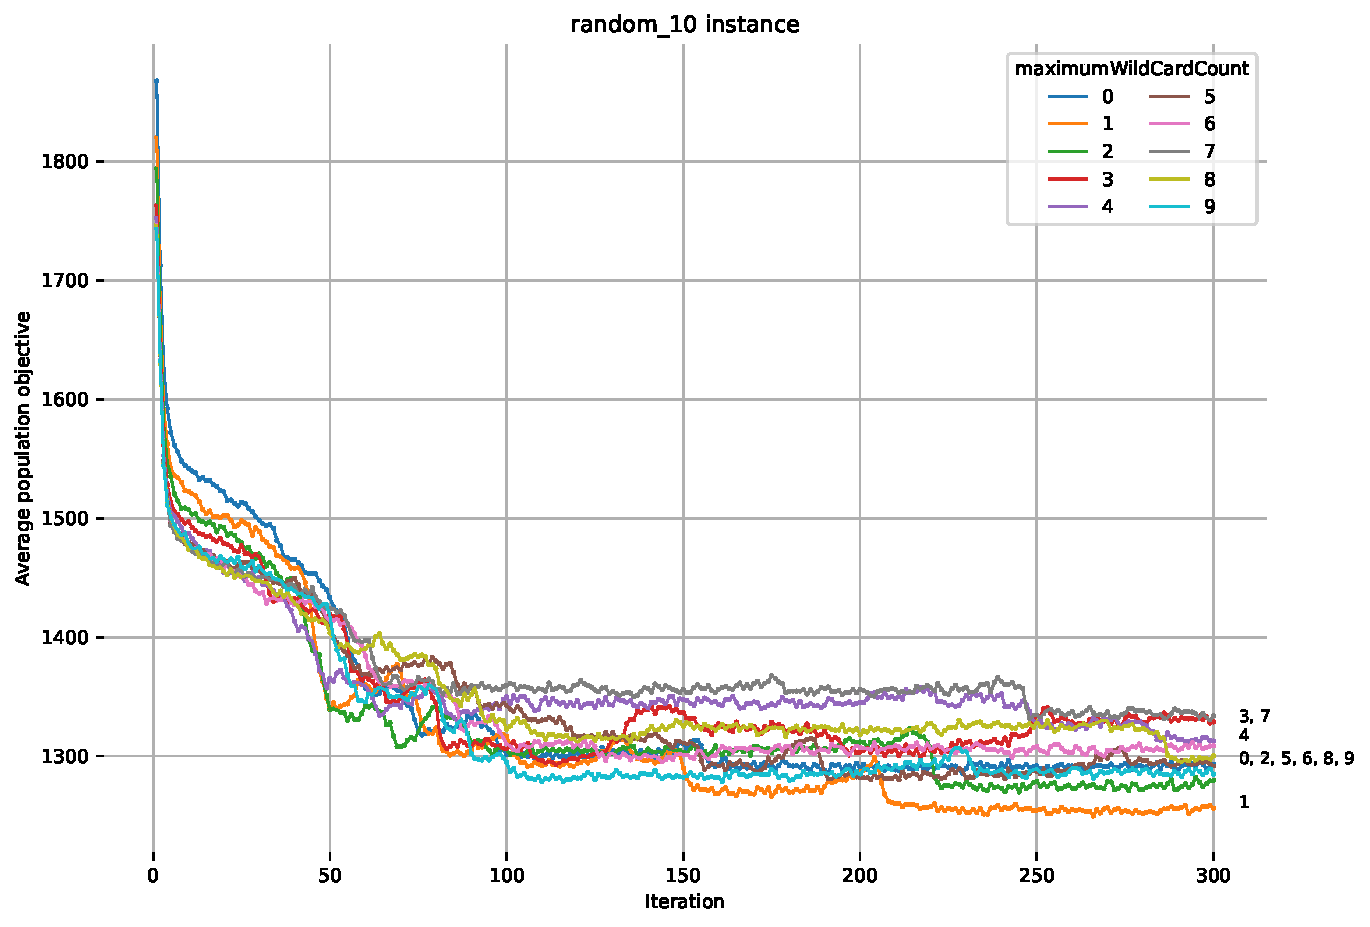
\includegraphics[width=1.1\textwidth]{hyperparameters/maximum_wild_card_count_performance_random_10}\label{subfig:hyperparams-maximum-wild-card-count-performance}}

    \subfloat{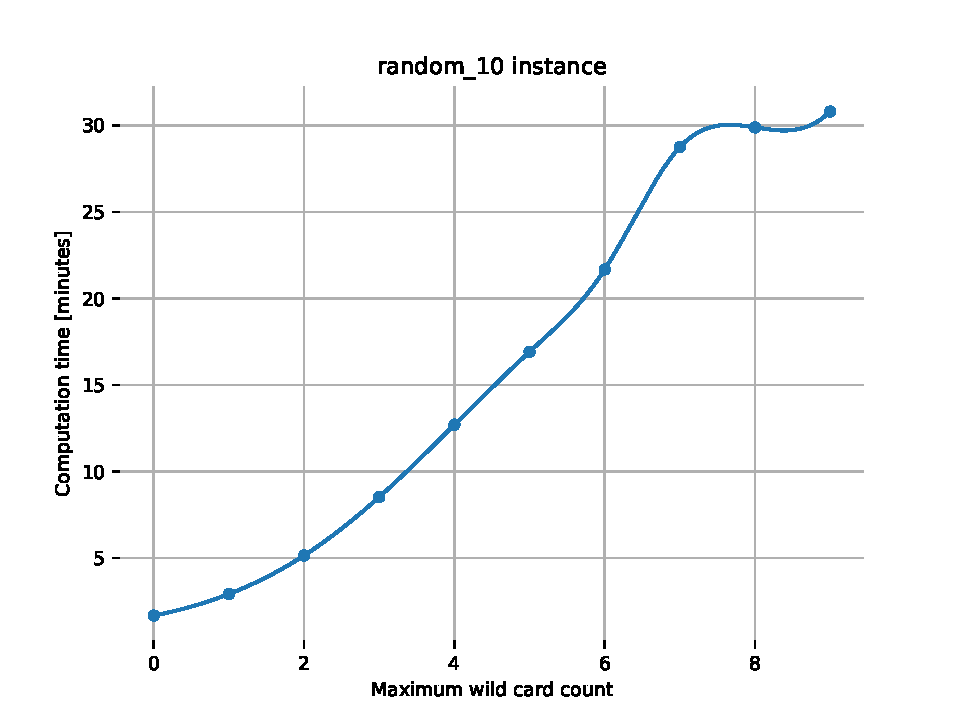
\includegraphics[width=0.8\textwidth]{hyperparameters/maximum_wild_card_count_computation_time_random_10}\label{subfig:hyperparams-maximum-wild-card-count-computation-speed}}
    \caption[Testing maximum wild card count]
    {Testing performance (top) and computation speed (bottom) for increasing maximum wild card count.}
    \label{fig:computation-time}%
\end{figure}
%    \end{landscape}
%    \clearpage% Flush page
%}

\afterpage{%
    \clearpage% Flush earlier floats (otherwise order might not be correct)
    \begin{landscape}% Landscape page
        \begin{figure}
            \centering
            \subfloat{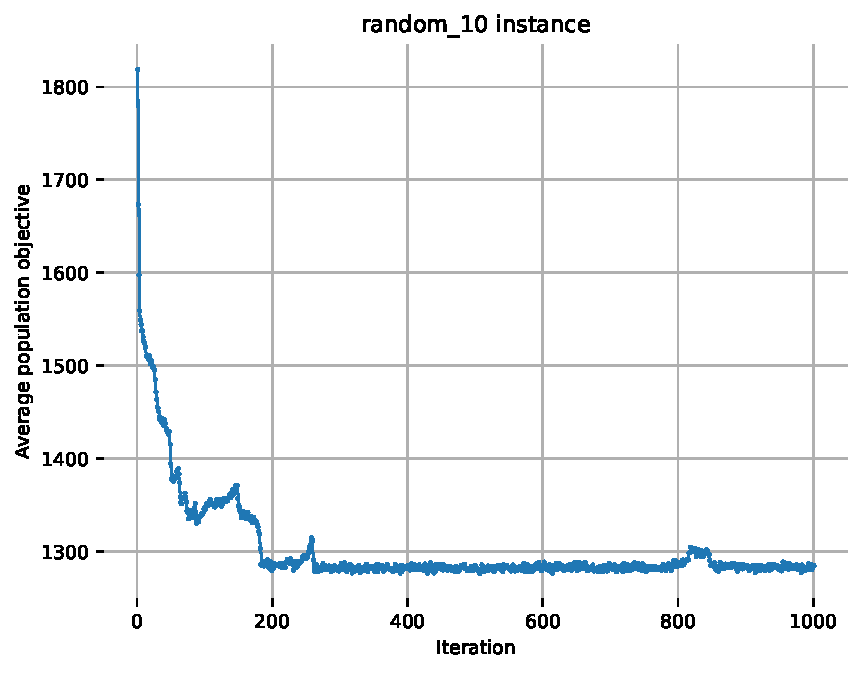
\includegraphics[width=0.8\textwidth]{hyperparameters/max_number_of_iter_random_10}\label{subfig:hyperparams-max-number-of-iter-random-10}}
            \subfloat{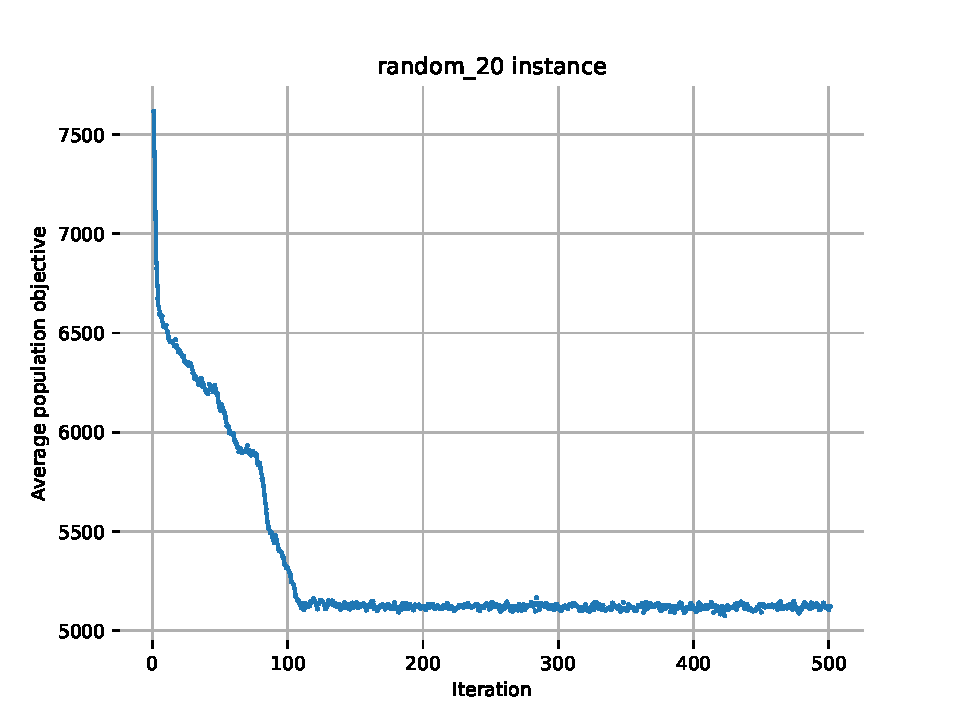
\includegraphics[width=0.8\textwidth]{hyperparameters/max_number_of_iter_random_20}\label{subfig:hyperparams-max-number-of-iter-random-20}}
            \caption[Testing maximum number of iterations]
            {Testing maximum number of iterations at two random instances.}
            \label{fig:hyperparams-max-number-of-iter}%
        \end{figure}
    \end{landscape}
    \clearpage% Flush page
}

\afterpage{%
    \clearpage% Flush earlier floats (otherwise order might not be correct)
    \begin{landscape}% Landscape page
        \begin{figure}
            \centering
            \subfloat{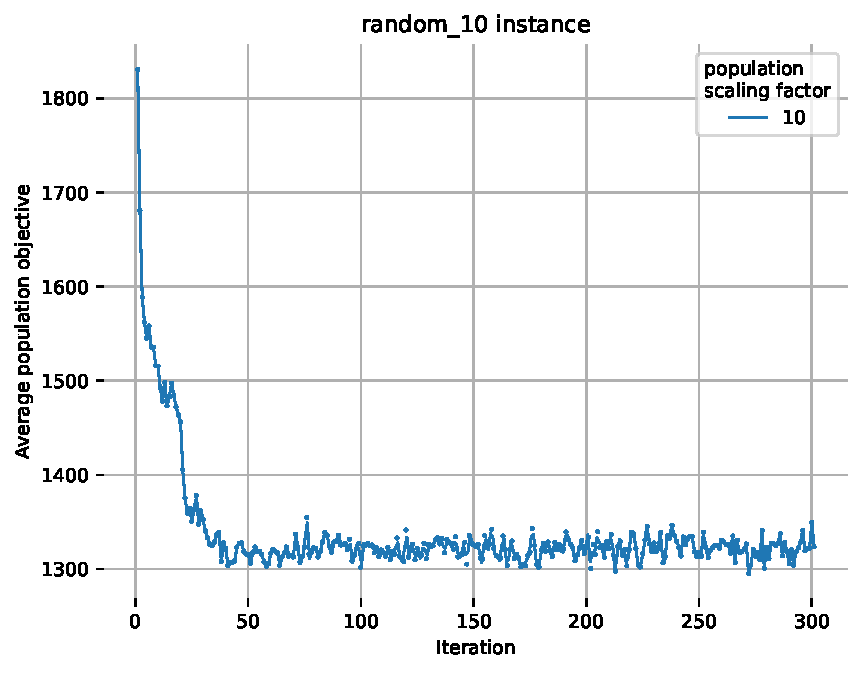
\includegraphics[width=0.8\textwidth]{hyperparameters/population_size_random_10}\label{subfig:hyperparams-population-size-random-10}}
            \subfloat{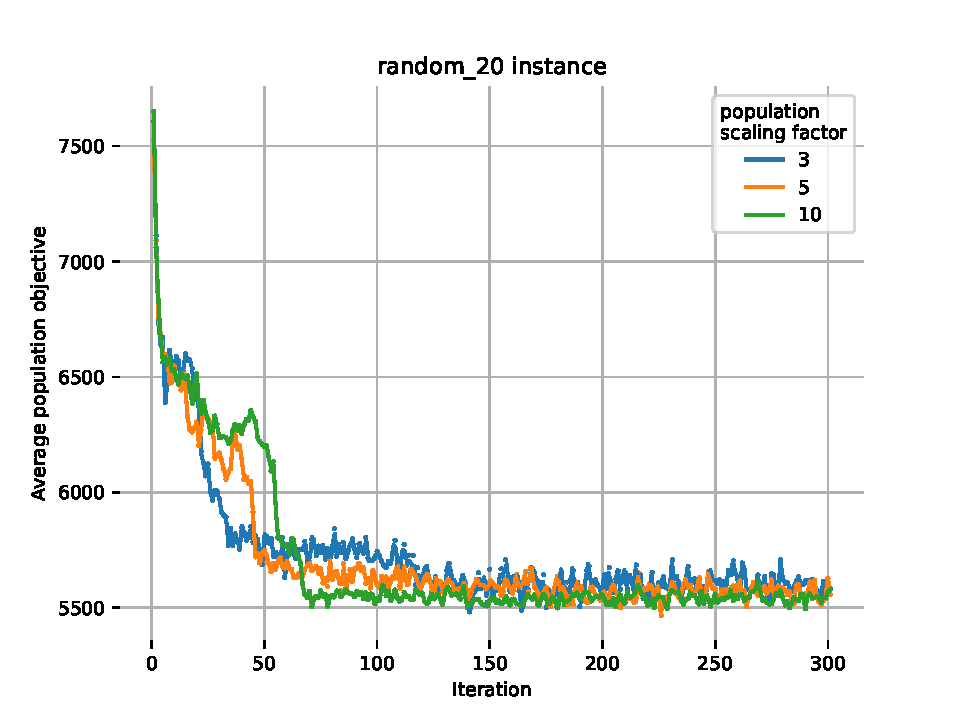
\includegraphics[width=0.8\textwidth]{hyperparameters/population_size_random_20}\label{subfig:hyperparameters-population-size-random-20}}
            \caption[Testing population scaling factor]
            {Testing population scaling factor at two random instances.
            The population size is $kN$ for population scaling factor $k$ and instance of size $N$. }
            \label{fig:hyperparameters-population-size}%
        \end{figure}
    \end{landscape}
    \clearpage% Flush page
}

\afterpage{%
    \clearpage% Flush earlier floats (otherwise order might not be correct)
    \begin{landscape}% Landscape page
        \begin{figure}
            \centering
            \subfloat{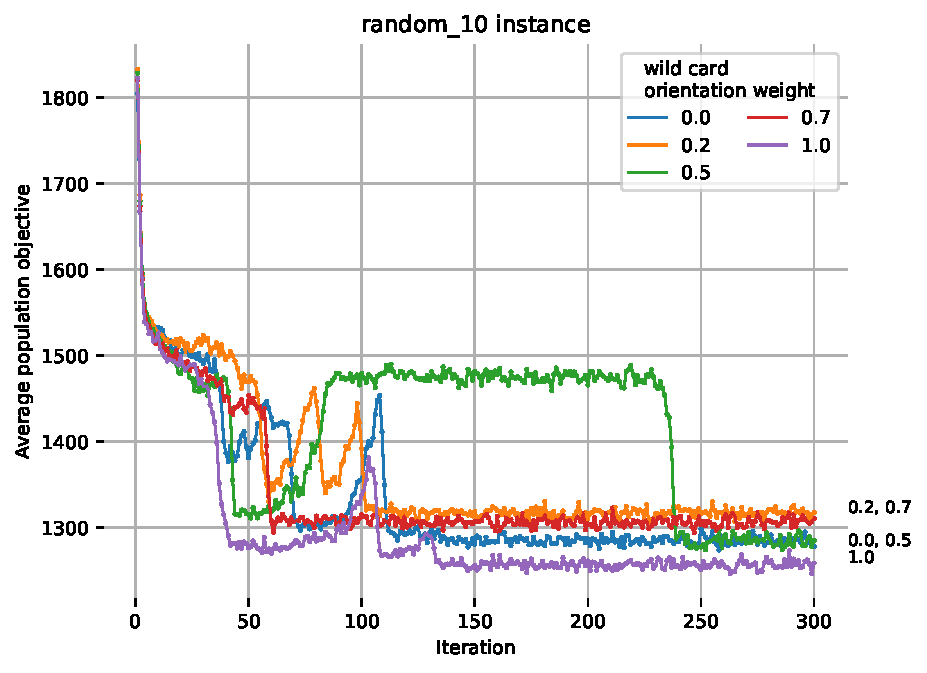
\includegraphics[width=0.8\textwidth]{hyperparameters/orientation_weights_random_10}\label{subfig:hyperparams-orientation-weights-random-10}}
            \subfloat{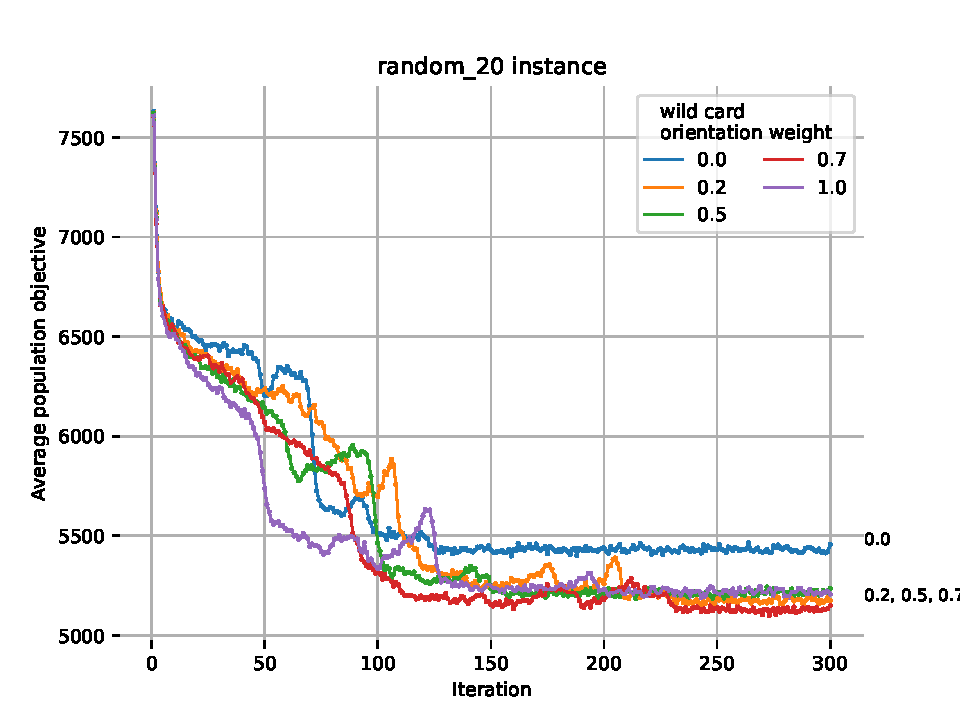
\includegraphics[width=0.8\textwidth]{hyperparameters/orientation_weights_random_20}\label{subfig:hyperparameters-orientation-weights-random-20}}
            \caption[Testing orientation weights]
            {Testing orientation weight for a wildcard cut type $*$ at two random instances.}
            \label{fig:hyperparameters-orientation-weights}%
        \end{figure}
    \end{landscape}
    \clearpage% Flush page
}

\afterpage{%
    \clearpage% Flush earlier floats (otherwise order might not be correct)
    \begin{landscape}% Landscape page
        \begin{figure}
            \centering
            \subfloat{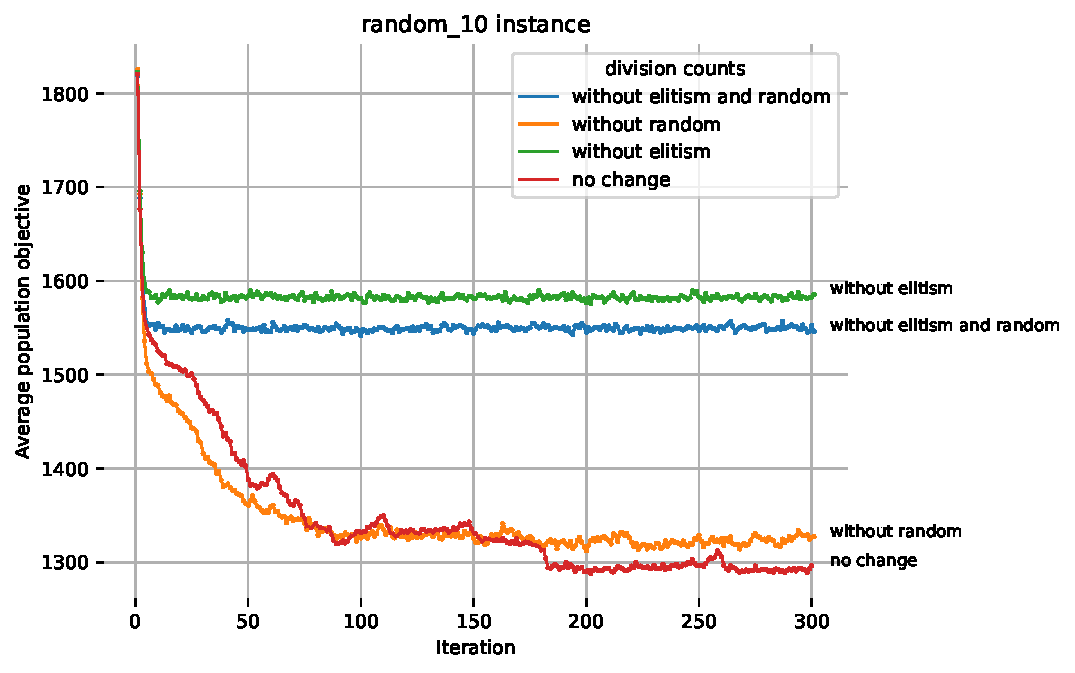
\includegraphics[width=0.8\textwidth]{hyperparameters/population_division_counts_random_10}\label{subfig:hyperparameters-population-division-counts-random-10}}
            \subfloat{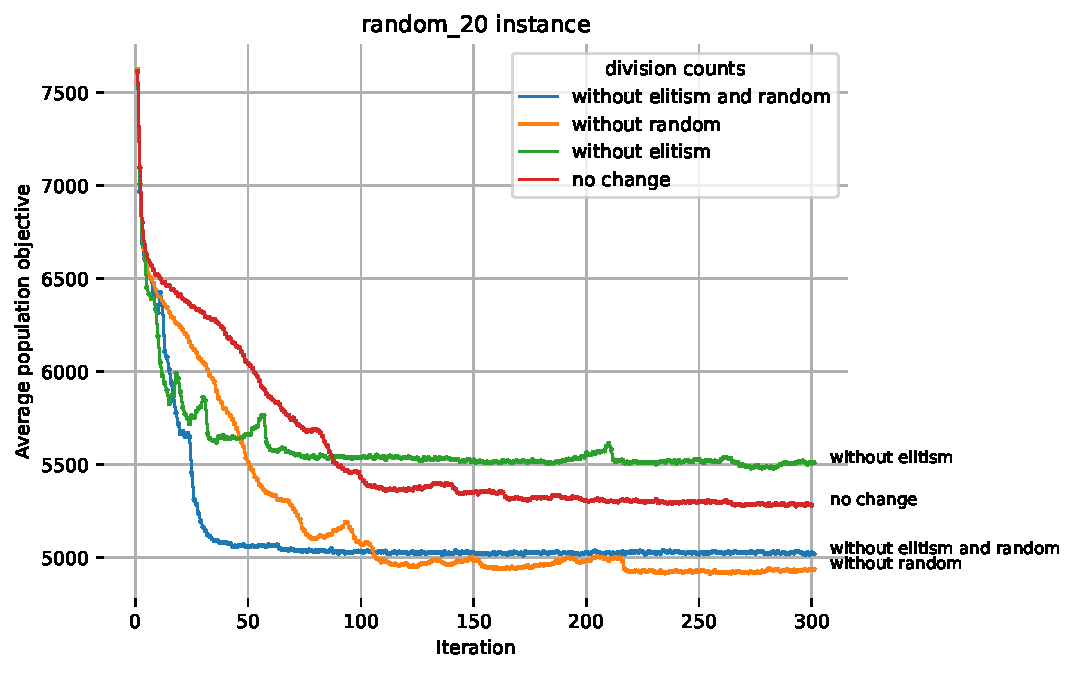
\includegraphics[width=0.8\textwidth]{hyperparameters/population_division_counts_random_20}\label{subfig:hyperparameters-population-division-counts-random-20}}
            \caption[Testing population division counts]
            {Testing population division counts at two random instances.
            Four variants are displayed. First does not use elitism, second does not inject random individuals, third combines first and second,
                and the last does not make any change to the population division counts.}
            \label{fig:hyperparameters-population-division-counts}%
        \end{figure}
    \end{landscape}
    \clearpage% Flush page
}

\afterpage{%
    \clearpage% Flush earlier floats (otherwise order might not be correct)
    \begin{landscape}% Landscape page
        \begin{figure}
            \centering
            \subfloat{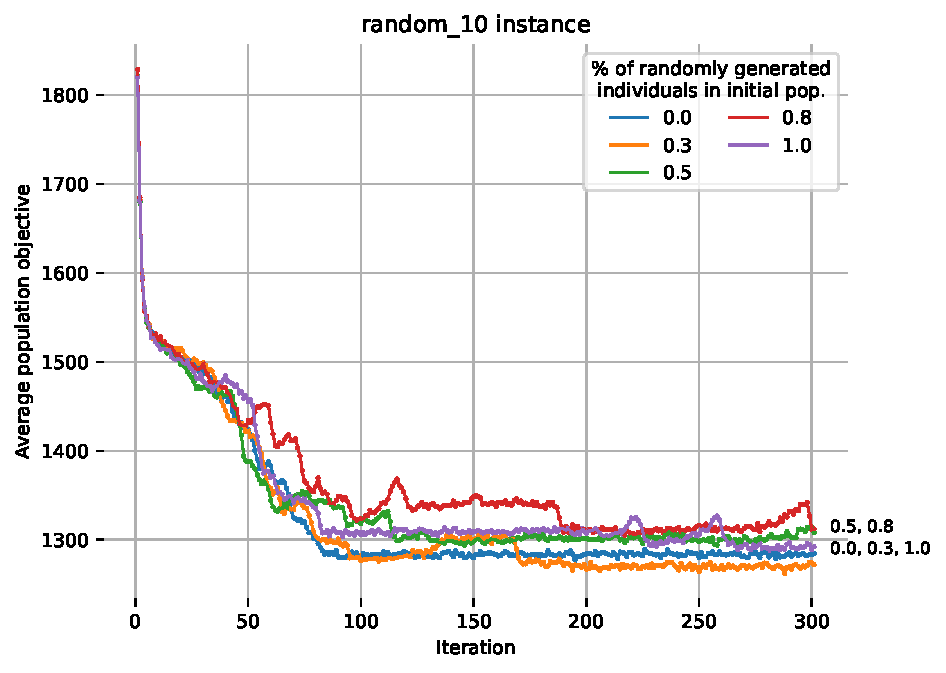
\includegraphics[width=0.8\textwidth]{hyperparameters/initial_population_division_counts_random_10}\label{subfig:hyperparameters-initial-population-division-counts-random-10}}
            \subfloat{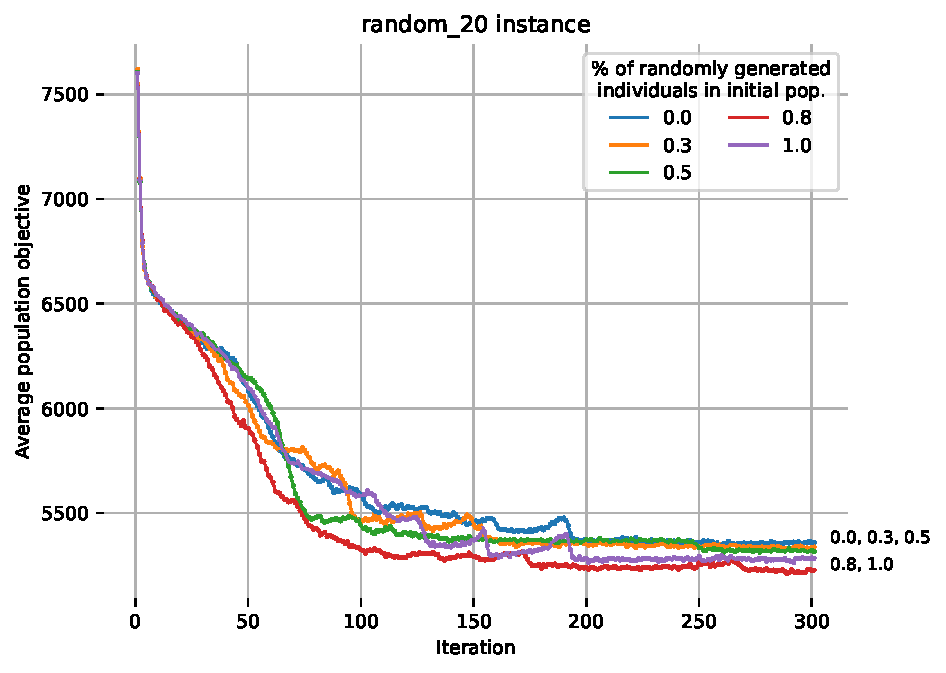
\includegraphics[width=0.8\textwidth]{hyperparameters/initial_population_division_counts_random_20}\label{subfig:hyperparameters-initial-population-division-counts-random-20}}
            \caption[Testing initial population division counts]
            {Testing initial population division counts at two random instances.}
            \label{fig:hyperparameters-initial-population-division-counts}%
        \end{figure}
    \end{landscape}
    \clearpage% Flush page
}

\afterpage{%
    \clearpage% Flush earlier floats (otherwise order might not be correct)
    \begin{landscape}% Landscape page
        \begin{figure}
            \centering
            \subfloat{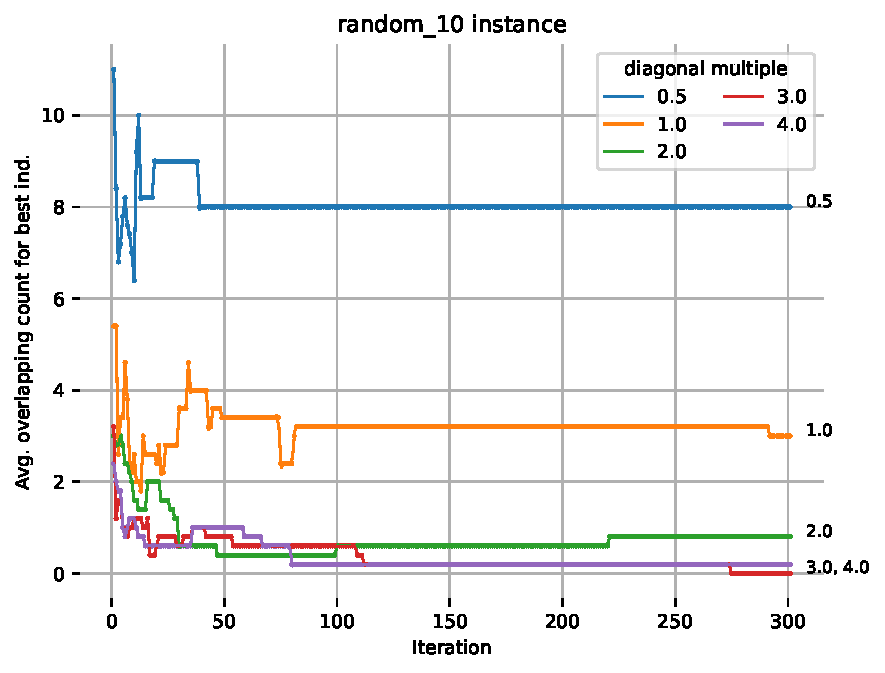
\includegraphics[width=0.8\textwidth]{hyperparameters/overlapping_penalization_constant_random_10}\label{subfig:hyperparameters-overlapping-penalization-constant-random-10}}
            \subfloat{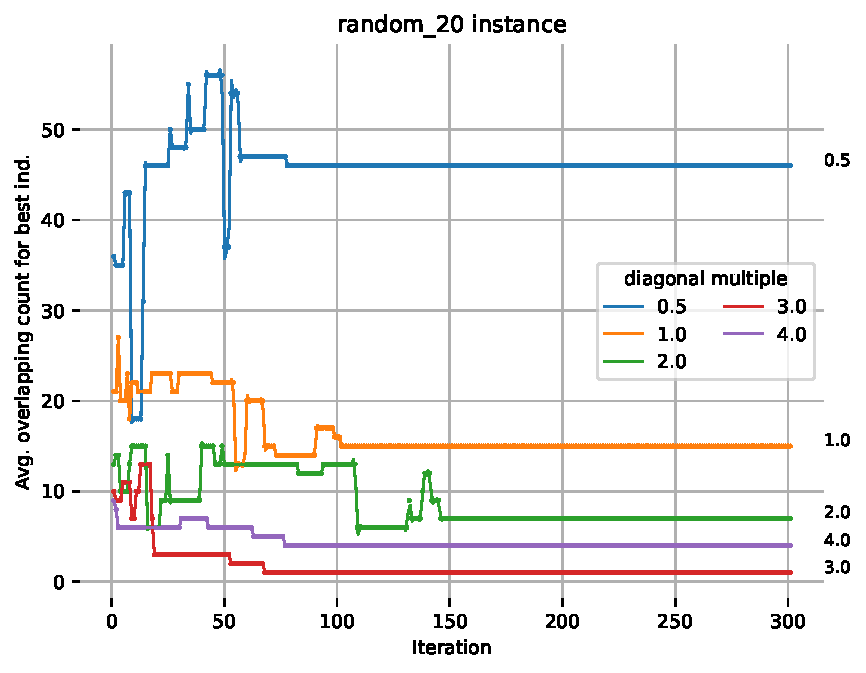
\includegraphics[width=0.8\textwidth]{hyperparameters/overlapping_penalization_constant_random_20}\label{subfig:hyperparameters-overlapping-penalization-constant-random-20}}
            \caption[Testing overlapping penalization constant]
            {Testing overlapping penalization constant $\lambda$ (eq.~\ref{eq:objective}) at two random instances.
            It is determined as $kD$, where $k$ is diagonal multiple and $D$ is the length of a diagonal in a layout.
            Graps show the average averlapping count for best individual at each iteration.}
            \label{fig:hyperparameters-overlapping-penalization-constant}%
        \end{figure}
    \end{landscape}
    \clearpage% Flush page
}

\afterpage{%
    \clearpage% Flush earlier floats (otherwise order might not be correct)
    \begin{landscape}% Landscape page
        \begin{figure}
            \centering
            \subfloat{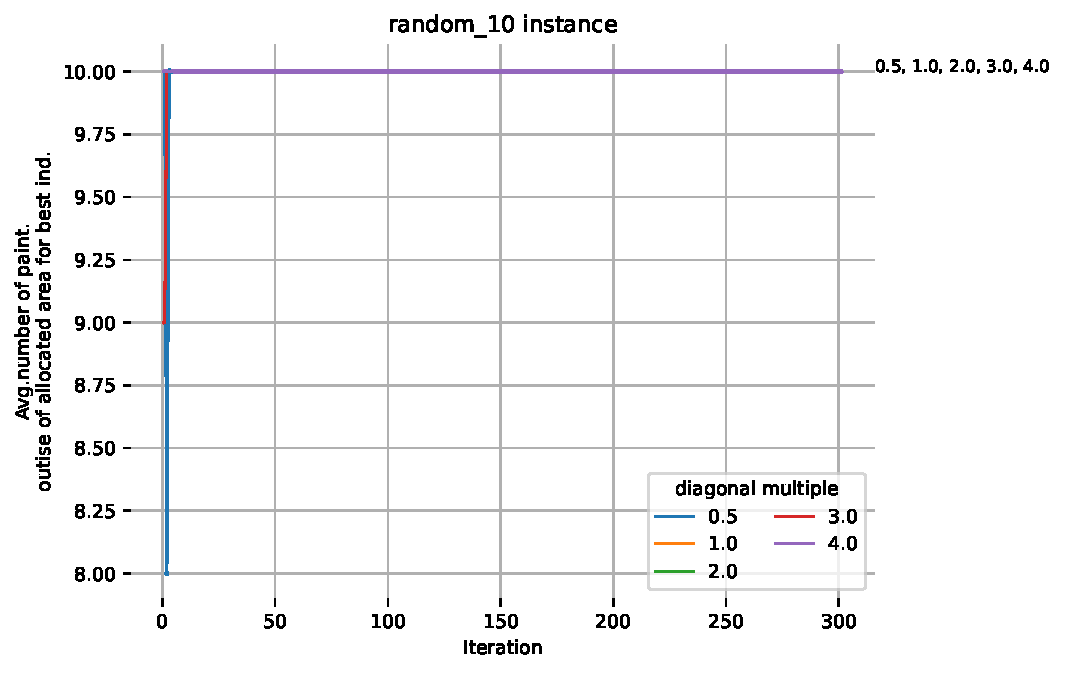
\includegraphics[width=0.8\textwidth]{hyperparameters/outside_of_allocated_area_penalization_constant_random_10}\label{subfig:hyperparameters-outside-of-allocated-area-penalization-constant-random-10}}
            \subfloat{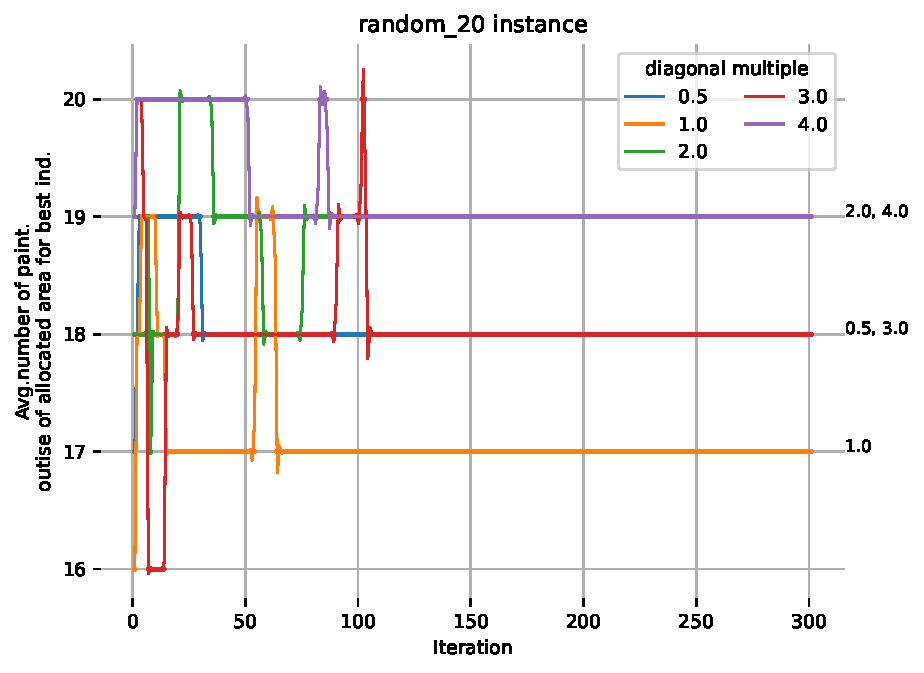
\includegraphics[width=0.8\textwidth]{hyperparameters/outside_of_allocated_area_penalization_constant_random_20}\label{subfig:hyperparameters-outside-of-allocated-area-penalization-constant-random-20}}
            \caption[Testing outside of allocated area penalization constant]
            {Testing outside of allocated area penalization constant $\gamma$ (eq.~\ref{eq:objective}) at two random instances.
            It is determined as $kD$, where $k$ is diagonal multiple and $D$ is the length of a diagonal in a layout.
            Graps show the average number of paintings that are placed outside of their allocated are for best individual at each iteration.}
            \label{fig:hyperparameters-outside-of-allocated-area-penalization-constant}%
        \end{figure}
    \end{landscape}
    \clearpage% Flush page
}

